\subsection{x86}

\subsubsection{\NonOptimizing MSVC}

\RU{Имеем в итоге}\EN{We get} (MSVC 2010):

\lstinputlisting[caption=MSVC 2010]{patterns/08_switch/2_lot/lot_msvc.asm.\LANG}

\index{jumptable}
\RU{Здесь происходит следующее: в теле функции есть набор вызовов \printf с разными аргументами. 
Все они имеют, конечно же, адреса, а также внутренние символические метки, которые присвоил им компилятор.
Также, все эти метки указываются во внутренней таблице \TT{\$LN11@f}.}
\EN{What we see here is a set of \printf calls with various arguments. 
All they have not only addresses in the memory of the process, but also internal symbolic labels assigned 
by the compiler. 
All these labels are also mentioned in the \TT{\$LN11@f} internal table.}

\RU{В начале функции, если $a$ больше 4, то сразу происходит переход на метку \TT{\$LN1@f}, 
где вызывается \printf с аргументом \TT{'something unknown'}.}
\EN{At the function start, if $a$ is greater than 4, control flow is passed to label 
\TT{\$LN1@f}, where \printf with argument \TT{'something unknown'} is called.}

\RU{А если $a$ меньше или равно 4, то это значение умножается на 4 и прибавляется адрес таблицы 
с переходами (\TT{\$LN11@f}). 
Таким образом, получается адрес внутри таблицы, где лежит нужный адрес внутри тела функции. 
Например, возьмем $a$ равным 2. $2*4 = 8$ (ведь все элементы таблицы ~--- это адреса внутри 32-битного процесса, 
таким образом, каждый элемент занимает 4 байта). 8 прибавить к \TT{\$LN11@f} ~--- это будет элемент таблицы,
где лежит \TT{\$LN4@f}. \JMP вытаскивает из таблицы адрес \TT{\$LN4@f} и делает безусловный переход туда.}
\EN{But if the value of $a$ is less or equals to 4, then it gets multiplied by 4 and added with the \TT{\$LN11@f} 
table address. That is how an address inside the table is constructed, pointing exactly to the 
element we need. For example, let's say $a$ is equal to 2. $2*4 = 8$ (all table elements 
are addresses in a 32-bit process and that is why all elements are 4 bytes wide). 
The address of the \TT{\$LN11@f} table + 8 will be the table element where the \TT{\$LN4@f} label is stored.
\JMP fetches the \TT{\$LN4@f} address from the table and jumps to it.}

\RU{Эта таблица иногда называется}\EN{This table is sometimes called} \IT{jumptable} \OrENRU 
\IT{branch table}\footnote{\EN{The whole method was once called}\RU{Сам метод раньше назывался} 
\IT{computed GOTO} \EN{in early versions of FORTRAN}\RU{В ранних версиях FORTRAN}:
\href{http://go.yurichev.com/17122}{wikipedia}.
\EN{Not quite relevant these days, but what a term}\RU{Не очень-то и полезно в наше время, но
каков термин}!}.

\RU{А там вызывается \printf с аргументом \TT{'two'}. 
Дословно, инструкция \TT{jmp DWORD PTR \$LN11@f[ecx*4]} 
означает \IT{перейти по DWORD, который лежит по адресу} \TT{\$LN11@f + ecx * 4}.}
\EN{Then the corresponding \printf is called with argument \TT{'two'}. 
Literally, the \TT{jmp DWORD PTR \$LN11@f[ecx*4]} instruction means
\IT{jump to the DWORD that is stored at address} \TT{\$LN11@f + ecx * 4}.}

\TT{npad} 
\ifx\LITE\undefined
(\myref{sec:npad})
\fi
\RU{это макрос ассемблера, немного выровнять начало таблицы, 
дабы она располагалась по 
адресу кратному 4 (или 16). Это нужно для того чтобы процессор мог эффективнее загружать 32-битное 
значения из памяти, через шину с памятью, кэш-память, и т.д.}
\EN{is assembly language macro that aligning the next label so that it will be stored at an address aligned on a 4 byte
(or 16 byte) boundary.
This is very suitable for the processor since it is able to fetch 32-bit values from memory through the memory bus,
cache memory, etc, in a more effective way if it is aligned.}

\ifdefined\IncludeOlly
\clearpage
\myparagraph{\olly}
\myindex{\olly}

\RU{Попробуем этот пример в}\EN{Let's try this example in} \olly.
\RU{Входное значение функции}\EN{The input value of the function} (2) \RU{загружается в}\EN{is loaded into} \EAX: 

\begin{figure}[H]
\centering
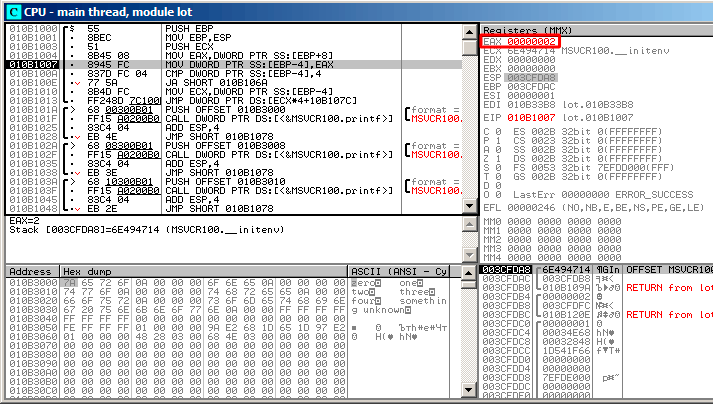
\includegraphics[scale=\FigScale]{patterns/08_switch/2_lot/olly1.png}
\caption{\olly: \RU{входное значение функции загружено в}\EN{function's input value is loaded in} \EAX}
\label{fig:switch_lot_olly1}
\end{figure}

\clearpage
\RU{Входное значение проверяется, не больше ли оно чем}\EN{The input value is checked, is it bigger than} 4? 
\RU{Нет, переход по умолчанию (\q{default}) не будет исполнен}\EN{If not, the \q{default} jump is not 
taken}:
\begin{figure}[H]
\centering
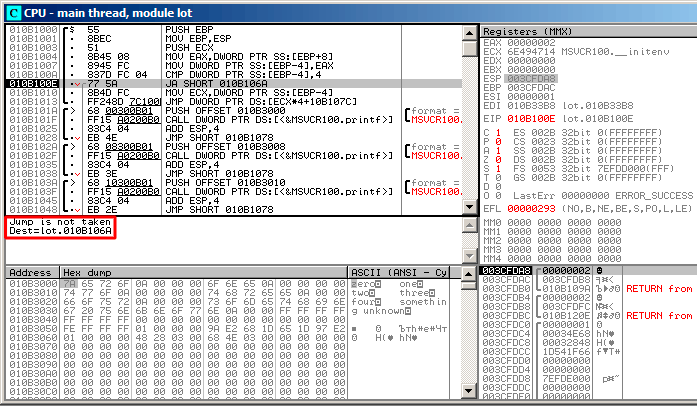
\includegraphics[scale=\FigScale]{patterns/08_switch/2_lot/olly2.png}
\caption{\olly: 2 \RU{не больше чем}\EN{is no bigger than} 4: \RU{переход не сработает}\EN{no jump is taken}}
\label{fig:switch_lot_olly2}
\end{figure}

\clearpage
\RU{Здесь мы видим}\EN{Here we see a} jumptable:

\begin{figure}[H]
\centering
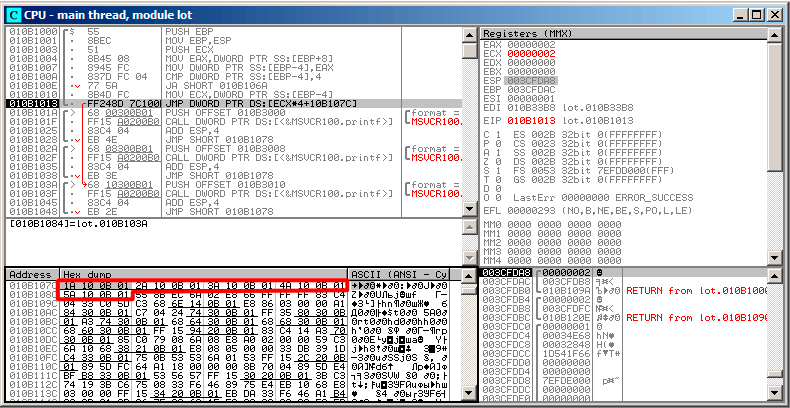
\includegraphics[scale=\FigScale]{patterns/08_switch/2_lot/olly3.png}
\caption{\olly: \RU{вычисляем адрес для перехода используя}\EN{calculating destination address using} jumptable}
\label{fig:switch_lot_olly3}
\end{figure}

\RU{Кстати, щелкнем по \q{Follow in Dump} $\rightarrow$ \q{Address constant}, так что теперь \IT{jumptable} видна в окне данных.}%
\EN{Here we've clicked \q{Follow in Dump} $\rightarrow$ \q{Address constant}, so now we see the \IT{jumptable} in the data window.}
\RU{Это 5 32-битных значений}\EN{These are 5 32-bit values}\footnote{\EN{They are underlined by \olly because
these are also FIXUPs}\RU{Они подчеркнуты в \olly, потому что это также и FIXUP-ы}: \myref{subsec:relocs}, 
\RU{мы вернемся к ним позже}\EN{we are going to come back to them later}}.
\ECX \RU{сейчас содержит}\EN{is now} 2\RU{, так что второй элемент (считая с нулевого) таблицы
будет использован}\EN{, so the second element (counting from zero) of the table is to be used}.
\RU{Кстати, можно также щелкнуть}\EN{It's also possible to click} \q{Follow in Dump} $\rightarrow$ 
\q{Memory address} \AndENRU \olly 
\RU{покажет элемент, который сейчас адресуется в инструкции \JMP}%
\EN{will show the element addressed by the \JMP instruction}. 
\RU{Это}\EN{That's} \TT{0x010B103A}.

\clearpage
\RU{Переход сработал и мы теперь на}\EN{After the jump we are at} \TT{0x010B103A}: 
\RU{сейчас будет исполнен код, выводящий строку}\EN{the code printing} \q{two}\EN{ will now be executed}:

\begin{figure}[H]
\centering
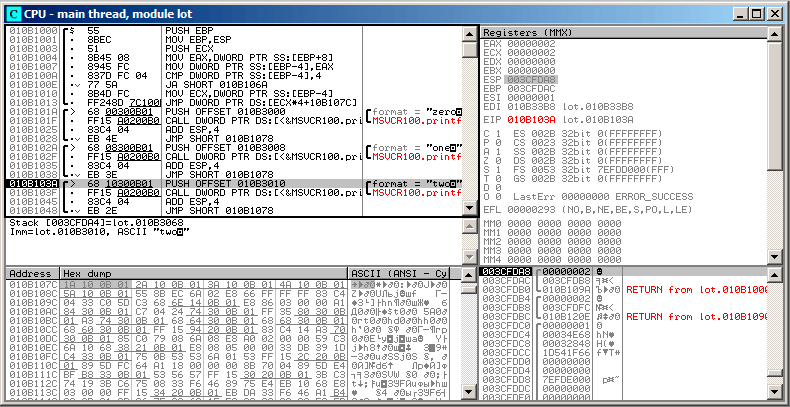
\includegraphics[scale=\FigScale]{patterns/08_switch/2_lot/olly4.png}
\caption{\olly: \RU{теперь мы на соответствующей метке}\EN{now we at the} \IT{case:}\EN{ label}}
\label{fig:switch_lot_olly4}
\end{figure}

\fi

\subsubsection{\NonOptimizing GCC}
\label{switch_lot_GCC}

\RU{Посмотрим, что сгенерирует GCC 4.4.1}\EN{Let's see what GCC 4.4.1 generates}:

\lstinputlisting[caption=GCC 4.4.1]{patterns/08_switch/2_lot/lot_gcc.asm}

\index{x86!\Registers!JMP}
\RU{Практически то же самое, за исключением мелкого нюанса: аргумент из \TT{arg\_0} умножается на 4 
при помощи сдвига влево на 2 бита (это почти то же самое что и умножение на 4)~(\myref{SHR}).
Затем адрес метки внутри функции берется из массива \TT{off\_804855C} и адресуется при помощи 
вычисленного индекса.}
\EN{It is almost the same, with a little nuance: argument \TT{arg\_0} is multiplied by 4 by
shifting it to left by 2 bits (it is almost the same as multiplication by 4)~(\myref{SHR}).
Then the address of the label is taken from the \TT{off\_804855C} array, stored in 
\EAX, and then \TT{``JMP EAX''} does the actual jump.}

